\documentclass[a4paper]{report}

\usepackage{amsmath}
\usepackage{amssymb}
\usepackage{amsthm}
\usepackage{tcolorbox} % for colorboxes
\usepackage{minted} % for code highlighting
\usepackage{xcolor} % for own colors
\usepackage[margin=3.8cm]{geometry} % custom page margin
\usepackage{algorithm} % pseudocode
\usepackage{algpseudocode} % pseudocode
\usepackage[german]{babel}
\usepackage{graphicx} % using images

\graphicspath{ {./assets/} } % setting the path for images

% LimeGreen!40
% blue!20
% purple!20
% orange!40
% Emerald!40

\definecolor{dcGrayLight}{gray}{0.95}
\definecolor{dcOrange}{RGB}{255, 128, 0}
\definecolor{dcGreen}{RGB}{117, 225, 102}
\definecolor{dcBlue}{RGB}{99, 203, 255}
\definecolor{dcRed}{RGB}{255,88,88}
\definecolor{dcWhite}{RGB}{255, 255, 255}
\colorlet{dcRedLight}{red!5!white}

\newtcolorbox{definition}[1][]{
    colframe=dcBlue,
    colback = white,
    coltitle = black,
    title = \textbf{Definition}
}

\newtcolorbox{lemma}[1][]{
    colframe=dcGreen,
    colback = white,
    coltitle = black,
    title = \textbf{Lemma}
}

\newtcolorbox{satz}[1][]{
    colframe=dcRed,
    colback = white,
    coltitle = black,
    title = \textbf{#1}
}

\setlength{\parindent}{0in} % remove indentation for paragraphs

\title{Algorithmen und Wahrscheinlichkeiten}
\author{Danny Camenisch (dcamenisch)}

\begin{document}
\maketitle
\tableofcontents
\listofalgorithms


% --------------------------
%   Templates and Examples
% --------------------------

\chapter{Template}
\section{tcolorbox}

\begin{definition}
    Definition...
\end{definition}

\begin{lemma}
    Lemma...
\end{lemma}

\begin{satz}[Satz von Danny]
    Satz...
\end{satz}

\begin{tcolorbox}[colback=dcWhite,colframe=dcOrange,title=\textbf{My Heading}]
    This is a \textbf{tcolorbox}.
\tcblower
    Here, you see the lower part of the box.
\tcbsubtitle{subtitle}
\end{tcolorbox}

\section{minted}

\begin{minted}[frame=lines, framesep=2mm, bgcolor=dcGrayLight, linenos]{java}
    // Hello.java
    import javax.swing.JApplet;
    import java.awt.Graphics;
    
    public class Hello extends JApplet {
        public void paintComponent(Graphics g) {
            g.drawString("Hello, world!", 65, 95);
        }    
    }
\end{minted}

% minted can also import from file like this:
% \inputminted{java}{main.java}


% --------------------------
%   Part 1.
% --------------------------
\part{Graphentheorie}
\chapter{Zusammenhang}

Wir erinnern uns an die Definition eines \textbf{zusammenhängenden} Graphen:

\begin{definition}
    Ein Graph $G = (V,E)$ heisst \textbf{zusammenhängend}, wenn $\forall u,v \in V, u \neq v$ 
    ein Pfad von u nach v in $G$ existiert. \\

    $X$ heisst \textbf{u-v-Seperator}, wenn u und v in verschiedenen Zusammenhangskomponenten von
    $G[V \backslash X]$ liegen.
\end{definition}
\bigskip

Diese Definition besagt zwar ob ein Graph zusammenhängend ist oder nicht, man kann aber nichts darüber sagen,
wie stark ein Graph zusammenhängend ist. Dafür definieren wir sowohl Knoten- als auch Kantenzusammenhang:

\begin{definition}
    Ein Graph $G = (V,E)$ heisst \textbf{k-zusammenhängend}, falls $|V| \geq k + 1$ und $\forall X \subseteq V$
    mit $|X| < k$ gilt: $G[V \backslash X]$ ist zusammenhängend. \\

    Ein Graph $G = (V,E)$ heisst \textbf{k-kanten-zusammenhängend}, falls $\forall X \subseteq E$
    mit $|X| < k$ gilt: $(V, E \backslash X)$ ist zusammenhängend.
\end{definition}
\bigskip

Ein Graph der 3-zusammenhängend ist, besitzt keine Seperator der Grösse 2 und ist dadurch auch 2-zusammenhängend. \\

Anschaulich zu merken: Wie viele Knoten oder Kanten muss man mindestens entfernen, bis der Graph nicht mehr
zusammenhängend ist.

\begin{lemma}
    Knoten-Zusammenhang $\leq$ Kanten-Zusammenhang $\leq$ minimaler Knotengrad
\end{lemma}
\bigskip

Ein (teils schwer zu beweisender) Satz erlaubt uns, eine äquivalente Definition von Zusammenhang
verwenden:

\begin{satz}[Satz von Menger]
    Sei $G = (V, E)$ ein Graph. Dann gilt:
    \begin{enumerate}
        \item $G$ ist k-zusammenhängend $\Leftrightarrow \forall u,v \in V, u \neq v$ gibt es mindestens k intern-knotendisjunkte u-v-Pfade.
        \item $G$ ist k-kanten-zusammenhängend $\Leftrightarrow \forall u,v \in V, u \neq v$ gibt es mindestens k intern-kantendisjunkte u-v-Pfade.
    \end{enumerate}
\end{satz}
\bigskip
\chapter{Artikulationsknoten und Brücken}

\begin{definition}
    Sei $G = (V,E)$ ein zusammenhängender Graph. Ein Knoten $v \in V$ heisst \textbf{Artikulationsknoten}
    (eng. cut vertex) genau dann wenn $G[V \backslash \{v\}]$ nicht zusammenhängend ist.
\end{definition}

\begin{definition}
    Sei $G = (V,E)$ ein zusammenhängender Graph. Eine Kante $e \in E$ heisst \textbf{Brücke}
    (eng. cut edge) genau dann wenn $G[E \backslash \{e\}]$ nicht zusammenhängend ist.
\end{definition}

\begin{lemma}
    Sei $G = (V,E)$ ein zusammenhängender Graph. Ist $\{x,y\} \in E$ eine Brücke so gilt für $x$
    (und analog auch für $y$): \\
    $$deg(x) = 1 \text{    oder    } x \text{ ist ein Artikulationsknoten}$$
\end{lemma}
\bigskip

Die Umkehrung ist hier aber nicht immer wahr! \\

Wie können wir nun solche Artikulationsknoten und Brücken finden? Dazu können
wir eine leicht modifizierte Version der bereits bekannten Tiefensuche verwenden. \\

Dazu müssen wir einige Beobachtungen machen. Zuerst, der von uns gewählte Startknoten $s$ der Tiefensuche,
und, für uns noch viel wichtiger, die Wurzel des Tiefensuchbaums $T$. Es wird schnell klar: Wenn $s$ im Tiefensuchbaum
eine Grad von mindestens 2 hat, so ist $s$ ein Artikulationsknoten. \\

Für jeden Knoten $v \neq s$ ist allerdings nicht so offensichtlich, ob $v$ ein Artikulationsknoten ist oder nicht.
Wieder können wir uns den Tiefensuchbaum zunutzen machen: $v$ ist ein Artikulationsknoten genau dann, wenn
$v$ im Baum Children (oder ganze Subtrees) besitzt, welche keine nicht-Baum-Kante zu einem Vorgänger von $v$ besitzen. \\

Um diese Voraussetzung zu überprüfen, definieren wir für unseren Graphen alle Kanten des Tiefensuchbaums als
\textit{Vorwärtskanten}, alle anderen als \textit{Rückwärtskanten}. Zusätzlich richten wir diese Kanten wie im Baum
(für Vorwärtskanten) bzw. vom höheren zum kleineren DFS Wert für Rückwärtskanten. Weiter definieren wir für jeden Knoten
$v \in V$: \\

low[v] $:=$ kleinste DFS-Nummer, die von $v$ aus durch einen Pfad mit beliebig vielen Vorwärtskanten und maximale
einer Rückwärtskante erreicht werden kann. \\

$
    \text{low}[v] = \text{ min} \left(
        \text{dfs}[v], \underset{(v,w) \in E}{\text{  min  }}
        \begin{cases}
            \text{dfs}[w], \text{ falls }(v,w) \text{ Restkante}\\
            \text{low}[w], \text{ falls }(v,w) \text{ Baumkante}
        \end{cases}
    \right)
$ \\
\\

Dann erhalten wir als Bedingung für Artikulationsknoten:

{\small 
\[
\text{v ist Artikulationsknoten} \Leftrightarrow
\begin{array}{l}
    v = s  v \text{ hat in } T \text{ Grad } \geq 2\\
    v \neq s \text{ und } \exists w \in V \text{ mit }\{v,w\} \in E(T) \wedge \text{ LOW[w]} \geq \text{DFS[v]}
\end{array}
\]
}

Wenden wir unser Wissen über Brücken an, so können wir diese im gleichen Zug berechnen: Eine gerichtete Kante 
${v, w}$ des Tiefensuchbaums (nur diese kommen in Frage) ist eine Brücke genau dann wenn low[$w$] $>$ dfs[$v$].
Restkanten sind niemals Brücken.\\

Unser angepasster DFS-Algorithmus sieht dann wie folgt aus, wobei als Input der Graph $G$ 
und der Startknoten $s$ verlangt wird:

\begin{algorithm}
    \caption{DFS(G,s)}
    \begin{algorithmic}[1]
        \State $\forall v \in V : \text{dfs}[v] \leftarrow 0$
        \State num $\leftarrow 0$ \Comment{Anzahl besuchter Knoten}
        \State $T \leftarrow \emptyset$ \Comment{Menge der Kanten im Tiefensuchbaum}
        \State \Call{DFS-Visit}{G,s}
        \If{\text{s hat in T mindestens Grad 2}}
            \State isArtVert[$s$] $\leftarrow$ TRUE
        \Else
        \State isArtVert[$s$] $\leftarrow$ FALSE
        \EndIf
    \end{algorithmic}
\end{algorithm}
\pagebreak
\begin{algorithm}
    \caption{DFS-Visit(G,v)}
    \begin{algorithmic}[1]
        \State num $\leftarrow$ num $ + 1$
        \State dfs[$v$] $\leftarrow$ num
        \State low[$v$] $\leftarrow$ dfs[$v$]
        \State isArtVert[$v$] $\leftarrow$ FALSE

        \For{$(v,w) \in E$}
            \If{dfs[$w$] $= 0$}
                \State $T \leftarrow T + (v,w)$
                \State val $\leftarrow$ \Call{DFS-Visit}{G,w} \Comment{low-Wert des direkten Nachfolgers}
                \If{val $\geq$ dfs[$v$]}
                \State isArtVert[$v$] $\leftarrow$ TRUE
                    \If{val $>$ dfs[$v$]}
                        \State isBridge[$v$][$w$] $\leftarrow$ TRUE
                    \EndIf
                \EndIf
                \State low[$v$] $\leftarrow$ min\{low[$v$], val\}
            \Else \Comment{Also ist dfs[$w$] $\neq 0$}
                \State low[$v$] $\leftarrow$ min\{low[$v$], dfs[$w$]\}
            \EndIf
        \EndFor

        \State \Return low[$v$]
    \end{algorithmic}
\end{algorithm}


\begin{satz}[Satz]
    In einem zusammenhängenden Graphen $G = (V,E)$, der als Adjazenzlist gespeichert ist, lassen sich
    alle Artikulationsknoten und Brücken in Zeit $\mathcal{O}(|E|)$ berechnen.
\end{satz}
\bigskip
\chapter{Block-Graphen}
\section{Blöcke}
\begin{definition}
    Sei $G = (V,E)$. Wir definieren eine Äquivalenzrelation auf $E$ wie folgt:
    $$e \sim f: \Leftrightarrow e = f \text{  oder  } \exists \text{ Kreis durch } e \text{ und } f$$
\end{definition}
\bigskip

Diese Äquivalenzklassen nennen wir auch \textbf{Blöcke}. Eine alternative Definition lautet wiefolgt:

\begin{definition}
    Sei $G = (V,E)$ ein zusammenhängender Graph. Ein \textbf{Block} ist eine maximale Menge von Kanten, so
    dass je zwei dieser Kanten auf einem gemeinsamen Kreis liegen.
\end{definition}
\bigskip

Merke: Ein Block ist ein Subgraph, der 2-zusammenhängend ist.

\begin{lemma}
    Zwei Blöcke schneiden sich - wenn überhaupt - immer in einem Artikulationsknoten.
\end{lemma}
\bigskip

Wir erinnern uns an die Definition von bipartiten Graphen.

\begin{definition}
    Ein Graph ist \textbf{bipartit}, wenn sich die Knotenmenge in zwei disjunkte Mengen
    $A$ und $B$ zerlegen lässt, sodass Kanten von $G$ nur zwischen $A$ und $B$ verlaufen.
    Wir verwenden dafür folgende Notation:
    $$V = A \uplus B$$
\end{definition}
\bigskip


\section{Block-Graphen}
Ein Block-Graph ist nun wiefolgt definitert:

\begin{definition}
    Der Block-Graph von $G$ ist der bipartite Graph $T = (A \uplus B, E_T )$ mit
    \begin{itemize}
        \item $A =$ {Artikulationsknoten von $G$}
        \item $B =$ {Blöcke von $G$}
        \item $\forall a \in A , b \in B: \{a,b\} \in E_T \Leftrightarrow a$ inzident zu einer Kante in $b$
    \end{itemize}
\end{definition}
\bigskip

\begin{figure}[h]
    \centering
    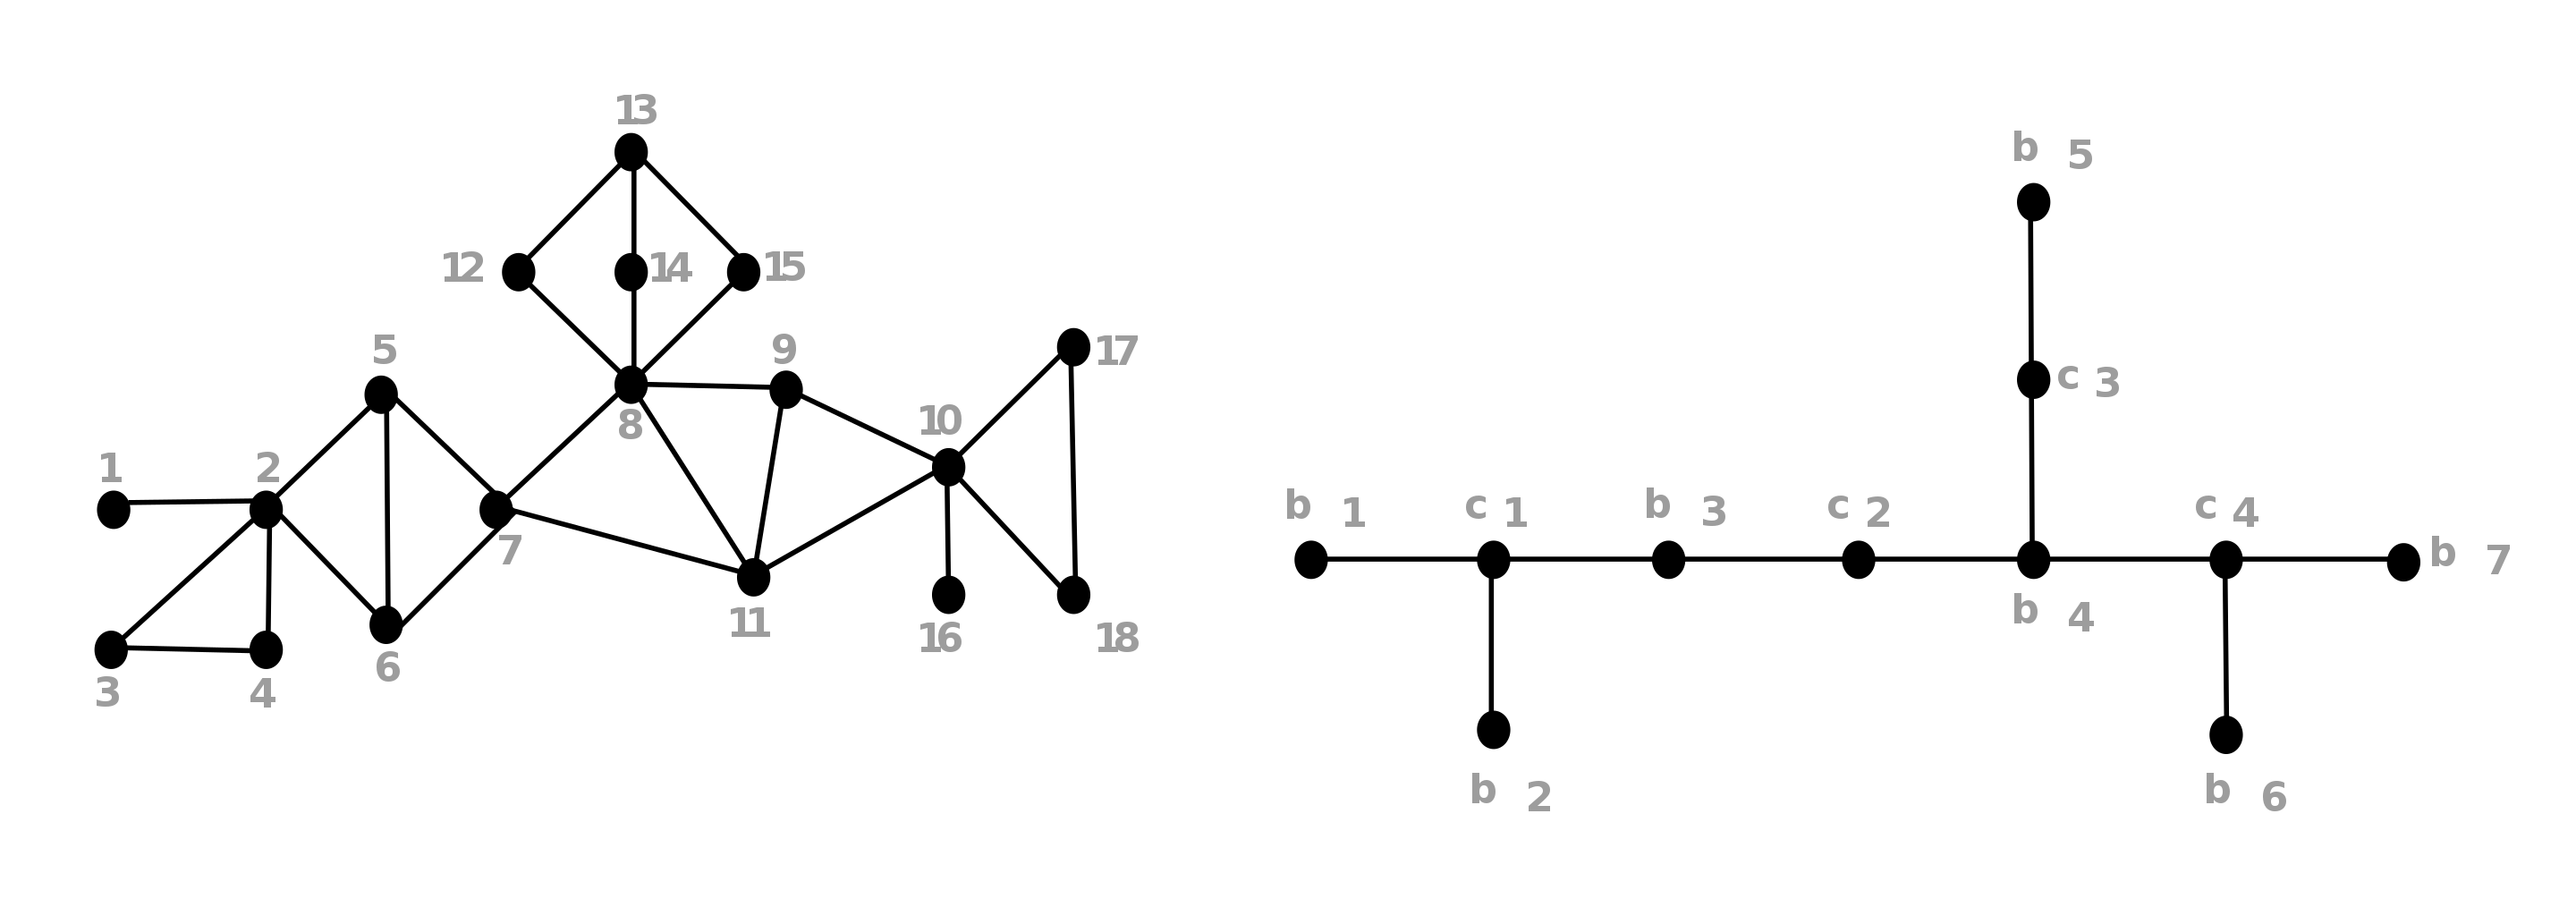
\includegraphics[width=\textwidth]{block_graph.png}
    \caption{Beispiel eines Graphen (links) und dem dazugehörigen Block-Graphen (rechts) }
\end{figure}
\chapter{Kreise}
\section{Eulertour}
\begin{definition}
    Sei $G = (V,E)$ ein Graph. Eine \textbf{Eulertour} ist ein geschlossener \text{Weg}, der jede Kante genau
    einmal enthält. Enthält ein Graph eine Eulertour, so nennt man ihn \textbf{eulersch}.
\end{definition}
\bigskip

Eine solche Tour lässt sich in $\mathcal{O}(|E|)$ finden - der Algorithmus (''schneller und langsamer Läufer'')
lässt sich ungefähr wie folgt beschreiben:

\begin{algorithm}
    \caption{Eulertour(G,s)}
    \begin{algorithmic}[1]
        \State $W \leftarrow$ \Call{Randomtour}{s} \Comment{''Läufer''}
        \State $v_{slow} \leftarrow $ Startknoten von $W$ \Comment{''Schildkröte''}
        \While{$v_{slow}$ ist nicht der letzte Knoten in $W$} 
            \State $v \leftarrow$ Nachfolger von $v_{slow}$ in $W$
            \If{$\exists (v,w) \in E, w \notin W$} \Comment{Ungenutze Kanten ab $v$}
                \State $W' \leftarrow$ \Call{Randomtour}{s}
                \State $W \leftarrow W_1 + W' + W_2$
            \EndIf
            \State $v_{slow} \leftarrow $ Nachfolger von $v_{slow}$ in $W$
        \EndWhile
        \Return $W$
    \end{algorithmic}
\end{algorithm}

\begin{algorithm}
    \caption{Randomtour(s)}
    \begin{algorithmic}[1]
        \State $v \leftarrow s$
        \State $W \leftarrow \{v\}$
        \While{$\exists (v,w) \in E, w \notin W$} \Comment{Ungenutze Kanten ab $v$}
            \State Wähle beliebigen Nachfolger $v_{next}$
            \State Hänge $v_{next}$ an $W$ analog
            \State $e \leftarrow \{v, v_{next}\}$
            \State Lösche $e$ aus $G$
            \State $v \leftarrow v_{next}$
        \EndWhile
        \State \Return $W$
    \end{algorithmic}
\end{algorithm}

Die Laufzeit ist leicht erklärt: Wir betrachten jede Kante genau einmal und ''löschen'' sie danach.

\begin{satz}[Satz]
    Ein zusammenhängender Graph $G = (V,E)$ enthält eine Eulertour $\Leftrightarrow$ der Grad jedes Knoten
    $v \in V$ ist gerade.
\end{satz}

\section{Hamiltonkreis}
\begin{definition}
    Sei $G = (V,E)$ ein Graph. Ein \textbf{Hamiltonkreis} ist ein Kreis, der alle Knoten von $V$ genau einmal
    durchläuft. Enthält ein Graph einen Hamiltonkreis, so nennt man ihn \textbf{hamiltonisch}.
\end{definition}
\bigskip

Ein klassisches Anwendungsbeispiel ist das Traveling Salesman Problem. Es wird vermutet, dass es keinen 
Algorithmus gibt, der in polynomieller Zeit bestimmt, ob es einen Hamiltonkreis in einem gegebenen Graphen 
gibt. \\

Es gibt aber einige Spezialfälle, für die es deutlich leichter ist, die Existenz eines Hamiltonkreises 
zu bestimmen:

\begin{itemize}
    \item Ein $n \times m$ Gitter enthält einen Hamiltonkreis genau dann wenn $n * m$ gerade ist
    \item Ein d-dimensionaler Hyperwürfel $H_d$ (Knotenmenge: $\{0, 1\}^d$, Kantenmenge: Alle Knotenpaare, welche sich in genau einer Koordinate unterscheiden) enthält einen Hamiltonkreis (auch für Dimensionen $d \geq 4$)
\end{itemize}

\begin{satz}[Satz von Dirac]
    Jeder Graph $G = (V, E)$ mit $|V| \geq 3$ und Minimalgrad $\delta(G) \geq |V| / 2$ enthält
    einen Hamiltonkreis. 
\end{satz}
\bigskip

Wenn wir einen Graphen anschauen, der nicht in einer dieser Kategorien fällt, wird es schwieriger um zu 
entscheiden, ob der Graph einen Hamiltonkreis enthält. Wenn wir das Problem mit Brute Force angehen, dauert
es $\mathcal{O}(n!)$. Nun wollen wir uns zwei Algorithmen anschauen, die etwas effizienter sind.

\pagebreak

\begin{algorithm}
    \caption{Hamiltonkreis(G)}
    \begin{algorithmic}[1]
        \For{$v \in [n]$ mit $v \neq 1$} \Comment{Initialisierung}
            \State $P_{(1,x), x} =
            \begin{cases}
                1, \text{ falls }(1,x) \in E\\
                0, \text{ sonst }
            \end{cases} $
        \EndFor

        \For{$s = 3$ bis $n$} \Comment{Initialisierung}
            \For{$S \subseteq [n]$ mit $1 \in S$ und $|S| = s$}
                \For{$x \in S, x \neq 1$}
                    \State $P_{s,x} = \text{max} \{ P_{S \backslash {x}, y}: y \in S \cap N(x), y \neq 1 \} $
                \EndFor
            \EndFor
        \EndFor

        \If{$\exists x \in N(1)$ mit $P_{[n],x} = 1$} \Comment{Ausgabe}
            \State \Return $G$ enthält einen Hamiltonkreis
        \Else
            \State \Return $G$ enthält keinen Hamiltonkreis
        \EndIf
    \end{algorithmic}
\end{algorithm}

Dieser Algorithmus kann in $\mathcal{O}(|V|^2 \cdot 2^{|V|})$ berechnen ob ein Hamiltonkreis existiert. Jedoch braucht
er dafür Speicherplatz in $\mathcal{O}(|V| \cdot 2^{|V|})$. Dies ist nicht optimal, daher gibt es einen zweiten Algorithmus,
der nicht nur die Existenz von Hamiltonkreisen feststellt, sondern auch gleich die Anzahl der Hamiltonkreise berechnet.

\begin{definition}
    $W_s = $ Anzahl der Wege der Länge $n$ von $s$ nach $s$ die keinen Knoten in $S \subset V$ besuchen. 
\end{definition}

\begin{algorithm}
    \caption{Zähle-Hamiltonkreis(G)}
    \begin{algorithmic}[1]
        \State $s = 1$ \Comment{Wahl des Startknoten (willkürlich)}
        \State $Z = |W_\emptyset|$
        \For{}
            \State Berechne $|W_S|$ \Comment{mit der Adjazenzmatrix von $G[V\backslash S]$}
            \State $Z = Z + (-1)^{|S|} \cdot |W_S|$
        \EndFor
        \State $Z = Z / 2$
        \State \Return $Z$ \Comment{Anzahl der Hamiltonkreise in $G$}
    \end{algorithmic}
\end{algorithm}

Dieser zweite Algorithmus hat eine Laufzeit von $\mathcal{O}(|V|^{2.81} \cdot \text{log}(|V|) \cdot 2^{|V|})$, braucht
dafür aber nur Speicherplatz in $\mathcal{O}(|V|^2)$, weshalb dieser Algorithmus in der Praxis meist besser ist. \\

Wir bemerken den drastischen Laufzeitunterschied gegenüber der Eulertour: Dort benötigten wir gerade 
einmal $\mathcal{O}(|E|)$ Zeit, um eine solche zu finden, während das Hamiltonkreisproblem nicht in polynomieller Zeit lösbar ist, da es 
NP-vollständig ist.

\section{NP-Probleme}

\begin{definition}
    Ein NP-Problem, ist ein Problem, dass nicht in polynomieller Laufzeit gelöst werden kann 
    (man nimmt es mindestens an). Das Gegenteil dazu sind P-Probleme.
\end{definition}

\section{Traveling Salesman}

Das Traveling Salesman Problem ist ein sehr berühmtes Problem:

\begin{definition}
    \textit{Gegeben sei ein vollständiger Graph mit n Knoten, berechne die kürzeste Rundreise.}
\end{definition}
\bigskip

Dies bedeutet effektiv, dass wir den minimalen Hamiltonkreis suchen. Das TSP ist stark mit dem Hamiltonkreisproblem
verwandt, aber wir haben nun statt einer binären Antwort, viele Antwortmöglichkeiten. Wir können aber aus dem TSP
ein Optimierungsproblem machen. Bezeichned opt$(K_n,l)$ die optimale Lösung für einen Graphen $K_n$ mit
Gewichtsfunktion $l$, so sprechen wir von einem $\alpha$-Approximationsalgorithmus, falls dieser immer eine 
Lösung $C$ mit
$$\sum_{e \in C} l(e) \leq \alpha \cdot \text{opt}(K_n, l)$$
findet. Allerdings sind wir so immernoch sehr eingeschränkt, denn wenn wir einen Graphen so konstruieren, dass
wir das Hamiltonkreisproblem lösen : Alle Kanten, die in einem anderen Graph (der zu untersuchen ist) vorkommen,
haben Gewicht 0. Da $\alpha \cdot 0 = 0$ müsste ein $\alpha$-Approximation immer einen Hamiltonkreis in seiner
Laufzeit finden. \\

Mithilfe einer zusätzlichen Annahme, können wir das TSP in aktzeptabler Laufzeit approximieren: Wir erwarten,
dass die Kantenlänge die \textit{Dreiecksungleichung} erfüllen, dass sich also Umwege nie lohnen würden. Wir
nenne dies, dass metrische TSP.

\begin{satz}[Satz]
    Für das metrische TSP gibt es einen 2-Approximationsalgorithmus mit Laufzeit $\mathcal{O}(n^2)$.
\end{satz}
\bigskip

Wir erreichen dies wie folgt: Wir berechne zuerst den MST des Graphen in $\mathcal{O}(n^2)$. Nun verdoppeln wir
alle Kanten - dadurch erhalten wir einen Weg von Länge $2 \cdot$ MST. Nun finden wir eine Eulertour, und durchlaufen
diese erneut, wobei wir 'Abkürzungen' verwenden, also keinen bereits besuchten Knoten erneut besuchen. Aufgrund der
Dreiecksungleichung wird unser Weg dadruch garantiert nicht länger. Da aus einem Hamiltonkreis durch entfernen einer
Kante ein Spannbaum wird, muss offensichtlich gelten dass
$$\text{MST}(K_n,l) \leq \text{opt}(K_n,l)$$
Insbesondere muss also die Länge unseres gefundenen Hamiltonkreises kleiner sein als $2 \cdot$ MST, und damit kleiner
als $2 \cdot$ opt, was ja genau zu zeigen war.
\input{chapters/traveling_salesman.tex}
\chapter{Matching}

Viele Zuordnungsprobleme lassen sich als ein Graphenproblem modellieren. Nehmen wir etwa an, wir müssen 
Jobs auf Rechner verteilen, aber nicht alle Rechner können alle Jobs ausführen. Modellieren wir dies durch 
einen Graphen, wobei Jobs und Rechner durch Knoten dargestellt sind, und Kanten zwischen Job und Rechner 
bedeuten das Erfüllen der Vorraussetzungen für den Job. Nun suchen wir eine Zuordnung, die möglichst jedem 
Job einen Rechner und jedem Rechner einen Job (der ausgeführt werden kann) zuordnet.

\begin{definition}
    Eine Kantenmenge $M \subseteq E$ heisst \textbf{Matching} in einem Graphen $G = (V,E)$, falls kein
    Knoten des Graphen zu mehr als einer Kante aus $M$ inzident ist, oder formal ausgedrückt, wenn
    $$e \cap f = \emptyset \text{    für alle    } e,f \in M \text{    mit    } e \neq f$$
    Ein Knoten $v$ wir von $M$ \textbf{überdeckt}, falls eine Kante $e \in M$ gibt, die $v$ enthält. \\

    Ein Matching $M$ heisst \textbf{perfektes Matching}, wenn jeder Knoten durch genau eine Kante aus
    $M$ überdeckt wird, oder, anders ausgedrückt, wenn $|M| = \frac{|V|}{2} $.
\end{definition}
\bigskip

Wir intressieren uns oft dafür, ein möglichst grosses Matching zu finden. Hierfür müssen wir definieren, was ein
möglichst grosses Matching ist:

\begin{definition}
    Sei $G = (V,E)$ ein Graph mit einem Matching $M$.
    \begin{itemize}
        \item $M$ heisst \textbf{inklusionsmaximal}, wenn es kein Matching $M'$ mit $M \subseteq M'$ und $|M| < |M'|$ gibt.
        \item $M$ heisst \textbf{kardinalitätsmaximal} (oder nur maximal), wenn es kein Matching mit $|M| < |M'|$ gibt.
    \end{itemize}
    Ein kardinalitätsmaximales Matching ist auch immer inklusionsmaximal, aber nicht umgekehrt. Weiter gilt,
    $|M_{inc}| \geq |M_{max}| / 2$. Haben wir ein kardinalitätsmaximal Matching mit $M = |V| / 2$, überdeckt es also alle
    Knoten, so nenne wir es ein \textbf{perfektes Matching}.
\end{definition}

\section{Matching-Algorithmen}

Wir schauen uns nun ein paar Algorithmen an, mitwelchen wir Matchings finden können.

\begin{algorithm}
    \caption{Greedy-Matching(G)}
    \begin{algorithmic}[1]
        \State $M \leftarrow \emptyset$
        \While{$E \neq \emptyset$}
            \State wähle eine beliebige Kante $e \in E$
            \State $ M \leftarrow M \cup \{e\}$
            \State lösche $e$ und alle inzidenten Kanten in $G$
        \EndWhile
        \State \Return $M$
    \end{algorithmic}
\end{algorithm}

Mit dem Greedy-Algorithmus kann in $\mathcal{O}(|E|)$ ein Matching bestimmt werden. Es gilt
$|M_{Greedy}| \geq |M_{max}| / 2$, wobei $M_{max}$ ein kardinalitätsmaximales Matching ist. \\

Solch ein Greedy-Matching muss nicht umbedingt ein kardinalitätsmaximales Matching sein. Wollen wir solche eines finden, dann
brauchen wir einen anderen Algorithmus. Dafür führen wir den Begriff des \textbf{augmentierenden Pfad} ein.
\begin{definition}
    Für ein Matching $M$, nennen wir eine Pfad \textbf{$M$-augmentierender}, wenn er abwechselnd Kanten
    aus $M$ und nicht aus $M$ enthält, und in (unterschiedlichen) Knoten die nicht von $M$ überdeckt werden startet und endet.
\end{definition}
\bigskip

Wenn wir solch einen $M$-augmentierenden Pfad $P$ haben, können wir durch tauschen der Zugehörigkeit aller Kanten im Pfad das Matching
vergrössern. Wir notieren das tauschen/augmentieren als $M \oplus P$.

\begin{satz}[Satz von Berger]
    Jedes Matching, das nicht kardinalitätsmaximal ist, besitz einen augmentierenden Pfad.
\end{satz}
\bigskip

Nun können wir einen simplen Algorithmus verwenden, um solch ein grösseres Matching zu erhalten. Wir schauen
uns hier nur den Algorithmus für bipartite Graphen an.

\begin{algorithm}
    \caption{Bipartite-Matching(G)}
    \begin{algorithmic}[1]
        \State $M \leftarrow \emptyset$
        \Repeat
            \State $P \leftarrow$ \Call{Augmenting-Path}{G,M}
            \State $M \leftarrow M \oplus P$
        \Until $P = \emptyset$
        \State \Return $M$
    \end{algorithmic}
\end{algorithm}

\pagebreak
Das Finden des augmentierenden Pfades erreichen wir durch modifizierte Breitensuche:

\begin{algorithm}
    \caption{Augmenting-Path(G = $(A \uplus B, E)$, M)}
    \begin{algorithmic}[1]
        \State $L_0 \leftarrow $\{unüberdeckte Knoten aus $A$\} und markiere $L_0$ als besucht
        \For{i = 1...n}
            \If{i ungerade}
                \State $L_i \leftarrow $ \{unbesuchte Nachbaren von $L_{i-1}$ via Kanten in $E \setminus M$ \}
            \Else 
                \State $L_i \leftarrow $ \{unbesuchte Nachbaren von $L_{i-1}$ via Kanten in $M$ \}
            \EndIf
            \State markiere Knoten aus $L_i$ als besucht
            \If{ein Knoten $v$ in $L_i$ nicht überdeckt ist}
                \State \Return Pfad von $L_0$ nach $v$ (backtracking)
            \EndIf
        \EndFor
    \end{algorithmic}
\end{algorithm}

Da BFS in $\mathcal{O}(|V| + |E|)$ läuft, und unser Matching maximal eine Grösse von $\frac{n}{2} = \mathcal{O}(n)$
hat, läuft unser Algorithmus in $\mathcal{O}(|V| \cdot |E|)$. Es ist einfach zu sehen, dass der kürzeste Pfad von
$L_0$ nach $v$ die Länge $i$ hat. \\

Wir können diesen Algorithmus aber noch etwas optimieren, so dass er in $\mathcal{O}(\sqrt{|V|} \cdot (|V| + |E|))$ läuft. Anstatt den erstbesten Pfad
zurückzugeben, suchen wir knotendisjunkte Pfade alle von unüberdeckten $v$ in $L_i$ nach $L_0$.

\begin{algorithm}
    \caption{Hopcroft-Karp(G)}
    \begin{algorithmic}[1]
        \State $M \leftarrow \emptyset$
        \Repeat
            \State $k \leftarrow$ länge eines kürzeste augmentierenden Pfades
            \State Finde alle disjunkte augmentierende Pfade $S$ der Länge $k$
            \For{Pfad P in S}
                \State $M \leftarrow M \oplus P$
            \EndFor
        \Until $P = \emptyset$
        \State \Return $M$
    \end{algorithmic}
\end{algorithm}
(\textit{Beweis siehe Vorlesung}) \\

Mit viel mehr Aufwand (randomisierte Algorithmen und lineare Programmierung) lassen sich andere effiziente Algorithmen finden,
die schneller und allgemeiner sind:
\begin{itemize}
    \item $\mathcal{O}(|V|^{1/2} \cdot |E|)$ für allgemeine Graphen
    \item $\mathcal{O}(|V|^{3})$ für gewichtete Graphen
\end{itemize}

\section{1.5-Approximation des TSP}

Der letztere Algorithmus ist insofern interessant, da wir dadurch eine 1.5-Approximation für das metrische TSP finden können.
Dies funktioniert ähnlich zur 2-Approximation:
\begin{enumerate}
    \item Berechne einen MST $T$ in $G$
    \item $U := \{\text{Knoten in $T$ mit ungeradem Grad}\}$, berechne ein perfektes Matching $M$ von $U$ mit minimalem Gewicht
    \item Füge $M$ zu $T$ hinzu, es entsteht ein Multigraph $T'$
    \item Berechne eine Eulertour $E$ in $T'$
    \item Kürze $E$ ab: überspringe Knoten die zum wiederholten mal besucht werden.
\end{enumerate}

\begin{satz}[Satz]
    Christofides' Algorithmus berechnet in Zeit $\mathcal{O}(|V|^{3})$ eine 1.5-Approximation für das metrische TSP.
\end{satz}
\bigskip

Seit September 2020 ist es möglich eine noch bessere Approximation zu finden \\ (1.4999999999999999999999999999999999990-Approximation). Dieser Durchbruch wird in den kommenden Jahren für
viele Verbesserungen sorgen.

\section{Satz von Hall}

\begin{definition}
    Ein Graph ist \textbf{regulär}, wenn alle Knoten den selben Grad haben.
\end{definition}

\begin{satz}[Satz von Hall (Heiratssatz)]
    Ein bipartiter Graph $G = (A \uplus B, E)$ enthält ein Matching $M$ der Kardinalität $|M| = |A|$, genau dann
    wenn $\forall X \subseteq A : |X| \leq |N(X)|$.
\end{satz}
\bigskip

Als direktes Korollar gibt es den Satz von Frobenius:

\begin{satz}[Satz von Frobenius]
    Für alle $k$ gilt: jeder $k$-reguläre, bipartite Graph enthält ein perfektes Matching.
\end{satz}
\bigskip

Dieses perfekte Matching lässt sich in Zeit $\mathcal{O}(|E|)$ bestimmen. Für $k=2^x$ ist dies leicht 
einzusehen: Wir bestimmen für jede Zusammenhangskomponente eine Eulertour. Dann entfernen wir jede 
zweite Kante davon, und erhalten einen $2^{x-1}$ regulären Graphen. Nach $x$ Iterationen ist der Graph
$2^0 = 1$ regulär, d.h. wir haben ein perfektes Matching gefunden. \\

Dies kann verallgemeinert werden, so dass es auch für nicht Zweierpotenzen funktioniert. Dies lassen 
wir hier aber aus.



% --------------------------
%   Part 2.
% --------------------------
\part{Wahrscheinlichkeiten}
\chapter{Die Siebformel}

\begin{satz}[Siebformel / Prinzip der Inklusion/Exklusion]
    Für endliche Mengen $A_1, A_2, ... , A_n$ mit $ n \geq 2$ gilt:
    $$\left\lvert \bigcup^{n}_{i = 1} A_i \right\rvert = \sum_{l = 1}^{n}(-1)^{l+1} \sum_{1 \leq i_1 < ... < i_l \leq n} \left\lvert A_{i_1} \cap ... \cap A_{i_l}\right\rvert$$
    In Worten: Alle Schnitte von einer \textit{ungeraden} Anzahl von Ereignissen \textit{addiert} man, alle Schnitte
    von einer \textit{geraden} Anzahl von Ereignissen \textit{substrahiert} man.
\end{satz}
\bigskip

Man kann sich diese Formel oft einfacher visualisieren als beschreiben: Auf folgender Grafik
kann man sich vergewissern, dass jede der sieben Teilmengen genau einmal gezählt wird:

\begin{figure}[h]
    \centering
    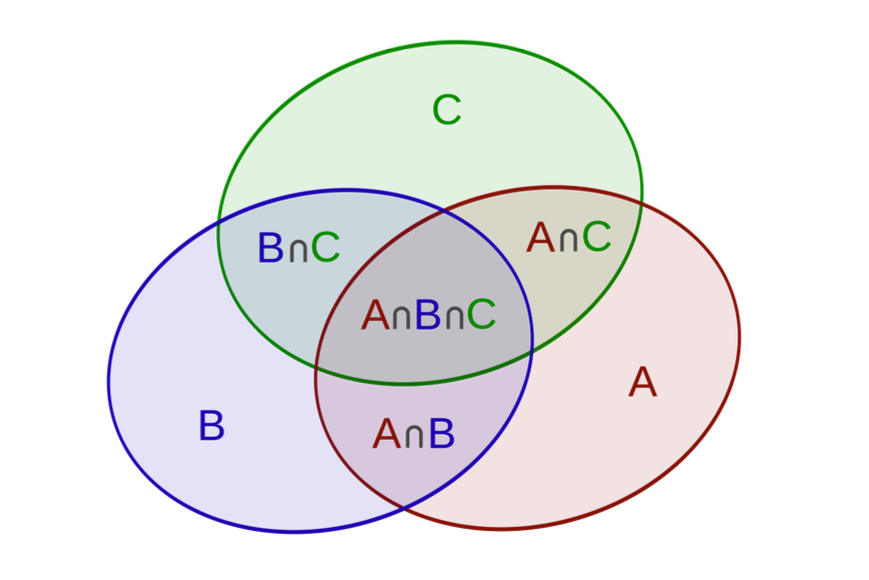
\includegraphics[width=9cm]{inclusion_exclusion.png}
    \caption{Beispiel Inklusion/Exklusion mit n = 3}
\end{figure}

$$\left\lvert \bigcup^{3}_{i = 1} A_i \right\rvert = \sum_{l = 1}^{3}\left\lvert A_l\right\rvert - \left\lvert A_1 \cap A_2 \right\rvert - \left\lvert A_2 \cap A_3 \right\rvert - \left\lvert A_1 \cap A_3 \right\rvert + \left\lvert A_1 \cap A_2 \cap A_3\right\rvert$$

\end{document}